%% Milestone 3 slides, group 38. Build: latexmk -pdf slides.tex
%% Every number comes from numbers.tex, which ms3.ipynb writes.
\documentclass[aspectratio=169,11pt]{beamer}
\usepackage{booktabs}
\usepackage{graphicx}
\usepackage[numbers,sort&compress]{natbib}
\usepackage{tikz}
\usetikzlibrary{arrows.meta,positioning,fit}
\graphicspath{{../../images/}}
% Written by ms3.ipynb; do not edit.
\newcommand{\nRows}{472,933}
\newcommand{\nTrain}{190,533}
\newcommand{\nValid}{76,487}
\newcommand{\nFeatures}{182}
\newcommand{\nHeavy}{72}
\newcommand{\nWeeks}{156}
\newcommand{\leakBound}{-0.001}
\newcommand{\shareStock}{22\%}
\newcommand{\shareWeek}{52\%}
\newcommand{\shareBoth}{74\%}
\newcommand{\icQ}{0.76}
\newcommand{\icW}{0.70}
\newcommand{\icMissTop}{har\_d}
\newcommand{\icMissTopValue}{-0.18}
\newcommand{\icEarn}{+0.17}
\newcommand{\nClusters}{55}
\newcommand{\nClustersAlpha}{50}
\newcommand{\evolvedTrain}{0.27}
\newcommand{\evolvedValid}{0.28}
\newcommand{\ridgeAlpha}{1000}
\newcommand{\lassoAlpha}{0.001}
\newcommand{\lassoKept}{102}
\newcommand{\lassoInputs}{383}
\newcommand{\qlikeHar}{0.209}
\newcommand{\mseHar}{0.367}
\newcommand{\ownFit}{83\%}
\newcommand{\stressTrain}{59}
\newcommand{\stressValid}{1}
\newcommand{\shareMissWeek}{37\%}
\newcommand{\corrDVix}{0.35}
\newcommand{\earnMiss}{+0.34}
\newcommand{\compTrain}{0.22}
\newcommand{\compValid}{0.21}
\newcommand{\singleTrain}{0.18}
\newcommand{\singleValid}{0.13}
\newcommand{\earnHar}{0.378}
\newcommand{\earnRidge}{0.214}
\newcommand{\noEarnHar}{0.192}
\newcommand{\highVixHar}{0.201}
\newcommand{\highVixMarket}{0.182}
\newcommand{\highVixRidge}{0.181}
\newcommand{\nHighVix}{8,640}
\newcommand{\mzHar}{0.96}
\newcommand{\mzRidge}{1.02}
\newcommand{\rHar}{0.54}
\newcommand{\rRidge}{0.61}
\newcommand{\stepLong}{-3.6\%}
\newcommand{\stepMarket}{-7.2\%}
\newcommand{\stepEarnings}{-13.0\%}
\newcommand{\stepAlpha}{-15.4\%}
\newcommand{\skewVar}{57}
\newcommand{\skewLog}{0.9}
\newcommand{\nFactors}{173}
\newcommand{\nNumeric}{181}
\newcommand{\evolvedTwoTrain}{-0.11}
\newcommand{\evolvedTwoValid}{-0.11}
\newcommand{\qLastWeek}{+28.3\%}
\newcommand{\mLastWeek}{+33.1\%}
\newcommand{\pLastWeek}{0.000}
\newcommand{\qStockMean}{+117.6\%}
\newcommand{\mStockMean}{+93.1\%}
\newcommand{\pStockMean}{0.000}
\newcommand{\qPooled}{+0.1\%}
\newcommand{\mPooled}{-0.4\%}
\newcommand{\pPooled}{0.890}
\newcommand{\qPooledFE}{-0.6\%}
\newcommand{\mPooledFE}{-1.6\%}
\newcommand{\pPooledFE}{0.441}
\newcommand{\qPooledMarket}{-2.0\%}
\newcommand{\mPooledMarket}{-2.2\%}
\newcommand{\pPooledMarket}{0.015}
\newcommand{\qGarch}{+24.9\%}
\newcommand{\mGarch}{+35.5\%}
\newcommand{\pGarch}{0.000}
\newcommand{\qRidge}{-15.5\%}
\newcommand{\mRidge}{-15.8\%}
\newcommand{\pRidge}{0.000}
\newcommand{\qLasso}{-15.6\%}
\newcommand{\mLasso}{-15.9\%}
\newcommand{\pLasso}{0.000}


\definecolor{accent}{HTML}{2A78D6}
\definecolor{target}{HTML}{E8853A}
\hypersetup{colorlinks, urlcolor=accent, linkcolor=., citecolor=accent}
\setbeamercolor{structure}{fg=accent}
\setbeamertemplate{bibliography item}[text]
\setbeamertemplate{frametitle continuation}{}
\setbeamertemplate{navigation symbols}{}
\setbeamertemplate{footline}{\hfill\insertframenumber\,/\,\inserttotalframenumber\hspace{1.5em}\vspace{0.8em}}
\setbeamerfont{frametitle}{size=\Large}
\newcommand{\speaker}[1]{\tikz[remember picture, overlay]
  \node[anchor=north east, xshift=-0.8em, yshift=-0.6em, font=\scriptsize, gray] at (current page.north east) {#1};}

\title{Forecasting Next-Week Volatility of S\&P 500 Stocks}
\subtitle{Milestone 3: EDA, baseline models and the modeling pipeline}
\author{Ashley Lee \and Juntang Wang \and Shuo Yang \and Simon Manivong \and Terry Su}
\institute{CS1090A / AC209A, Fall 2026 \quad Group 38, project 12 \quad TF: Daniel More Torres}
\date{}

\begin{document}

\begin{frame}
  \titlepage
\end{frame}

%% =================================================================
%% Recap
%% =================================================================
\begin{frame}{Where Milestone 2 left us \speaker{Ashley}}
  \begin{columns}[T]
    \column{0.55\textwidth}
    \textbf{Question}: for each S\&P 500 stock and week, forecast next week's log variance
    (Garman--Klass, from daily prices).
    \begin{enumerate}\setlength\itemsep{0.3em}
      \item \textbf{Accuracy}: do pooled models (ridge, lasso, then boosted trees) beat HAR
            fit stock by stock? QLIKE, MSE, Diebold--Mariano at 5\%.
      \item \textbf{Attribution}: which feature blocks carry the gain, in calm and in stress weeks?
    \end{enumerate}
    \vspace{0.3em}
    \textbf{Data}: \nRows{} stock-weeks $\times$ \nFeatures{} features in 10 blocks, each known at the
    Friday close; delisted stocks included.
    \column{0.42\textwidth}
    \footnotesize
    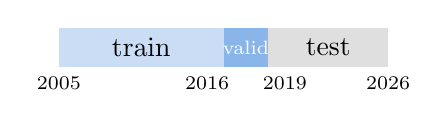
\begin{tikzpicture}[x=0.19cm, y=1cm]
      \fill[accent!25] (0,0) rectangle (11,0.5);
      \fill[accent!55] (11,0) rectangle (14,0.5);
      \fill[gray!25] (14,0) rectangle (22,0.5);
      \node at (5.5,0.25) {train};
      \node[white, font=\scriptsize] at (12.5,0.25) {valid};
      \node at (18,0.25) {test};
      \node[below, font=\scriptsize] at (0,0) {2005};
      \node[below left, font=\scriptsize, inner xsep=1pt] at (11.6,0) {2016};
      \node[below right, font=\scriptsize, inner xsep=1pt] at (13.4,0) {2019};
      \node[below, font=\scriptsize] at (22,0) {2026};
    \end{tikzpicture}\\[0.6em]
    \begin{itemize}\setlength\itemsep{0.3em}
      \item \textbf{This milestone} reads train and validation only; the test years stay sealed.
      \item EDA that drives a choice uses \textbf{training years only}.
      \item Every model is scored on the \textbf{same \nValid{} validation rows}.
    \end{itemize}
  \end{columns}
\end{frame}

%% =================================================================
%% EDA
%% =================================================================
\begin{frame}{EDA: most of the variance is common to a week \speaker{Juntang}}
  \begin{columns}[c]
    \column{0.5\textwidth}
    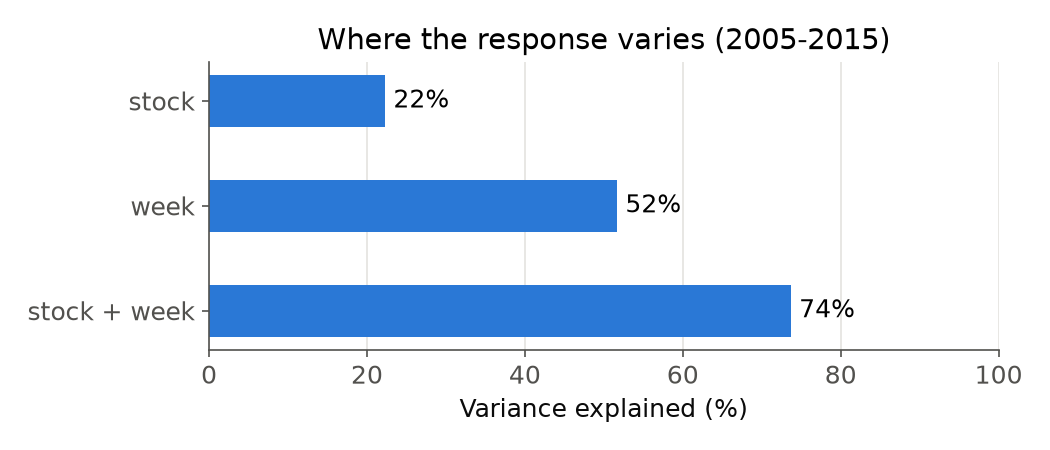
\includegraphics[width=\linewidth]{ms3_variance_decomposition.png}
    \column{0.48\textwidth}
    \small
    \begin{itemize}\setlength\itemsep{0.6em}
      \item \textbf{Log scale}: variance has skewness \skewVar{}, its log \skewLog{}. We fit the log; QLIKE gets
            $e^{\hat y}$ times Duan's smearing factor.
      \item \textbf{Week effects} explain \shareWeek{} of the target's variance, company effects
            \shareStock{}, both \shareBoth{}.
      \item \shareMissWeek{} of HAR's miss is common to a week; it tracks the change in VIX
            ($r = \corrDVix$).
      \item \textbf{So}: market information may matter as much as pooling. The baselines climb
            Zhang et al.'s ladder~\citep{zhang2024commonality}: per stock, pooled, pooled + market.
    \end{itemize}
  \end{columns}
\end{frame}

\begin{frame}{EDA: factor research, the way a quant desk scores signals \speaker{Juntang}}
  \begin{columns}[c]
    \column{0.6\textwidth}
    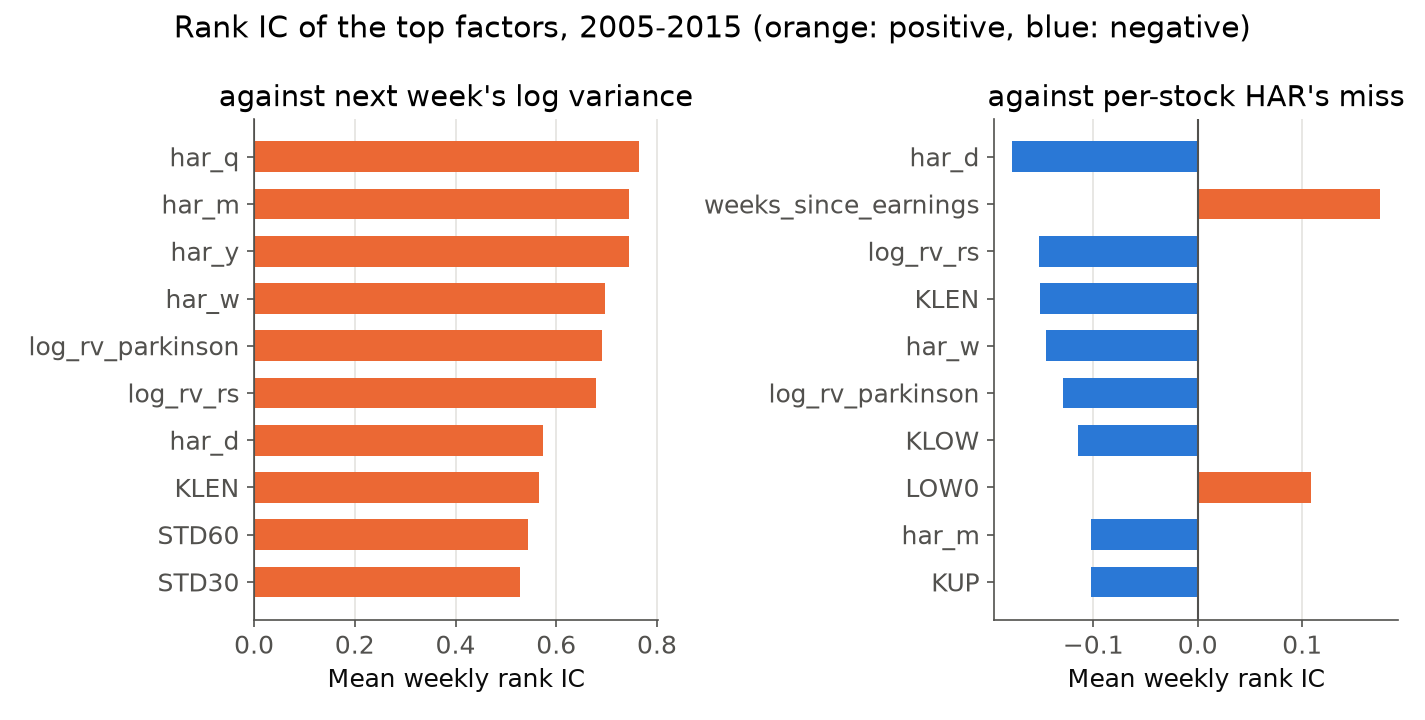
\includegraphics[width=\linewidth]{ms3_factor_ic.png}
    \column{0.38\textwidth}
    \footnotesize
    \textbf{Rank IC}: correlation across stocks within a week, averaged over weeks~\citep{grinold2000active}.
    \begin{itemize}\setlength\itemsep{0.4em}
      \item \textbf{Left}: the quarterly lag ranks stocks best (IC \icQ{}, last week \icW{}).
      \item \textbf{Right}, against HAR's miss: a high last day lands below HAR's forecast
            (IC \icMissTopValue{}); weeks since earnings \icEarn{}: HAR cannot see the
            earnings bump (\earnMiss{} in log variance).
      \item \textbf{So}: long memory, earnings and candle factors are the blocks expected to add
            to HAR.
    \end{itemize}
  \end{columns}
\end{frame}

\begin{frame}{EDA: factors are stable, many, and can be evolved \speaker{Juntang}}
  \begin{columns}[c]
    \column{0.47\textwidth}
    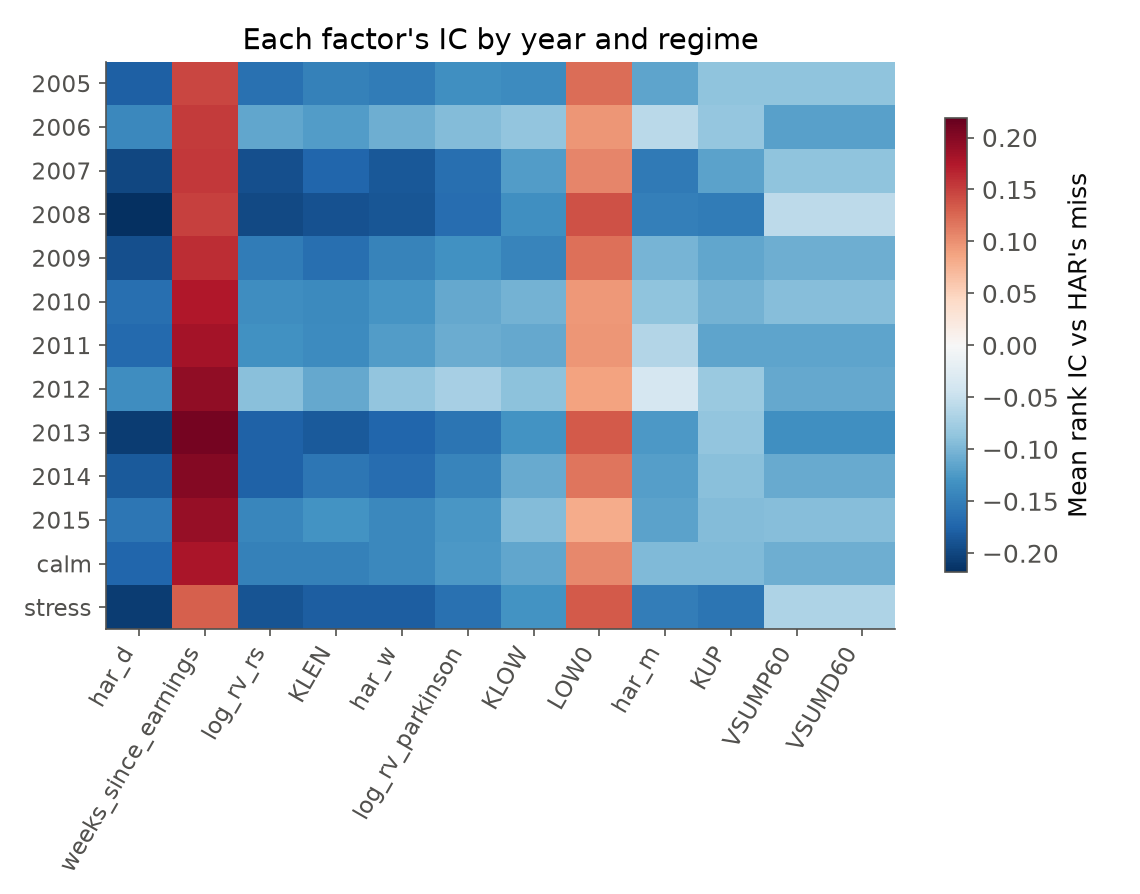
\includegraphics[width=\linewidth]{ms3_factor_evolution.png}
    \column{0.51\textwidth}
    \small
    \begin{itemize}\setlength\itemsep{0.55em}
      \item \textbf{Evolution over time}: none of the top 12 flips sign in any year 2005--2015.
      \item \textbf{Multi-factor}: \nFactors{} factors form \nClusters{} clusters (Alpha158: \nClustersAlpha{}).
            A composite of the cluster leaders has IC \compTrain{} in training and
            \compValid{} on validation, against \singleTrain{} and \singleValid{} for the best
            single factor.
      \item \textbf{Factor evolution} by genetic programming~\citep{koza1992gp,stephens2026gplearn}:
            the best formula is $\text{har}_q - \text{har}_d + \sqrt{\text{weeks since earnings}}$,
            IC \evolvedTrain{} in training, \evolvedValid{} on validation.
      \item \textbf{So}: many weak signals that add up out of sample: the case for a pooled model
            on every block.
    \end{itemize}
  \end{columns}
\end{frame}

\begin{frame}{EDA decides the preprocessing \speaker{Shuo}}
  \begin{columns}[c]
    \column{0.4\textwidth}
    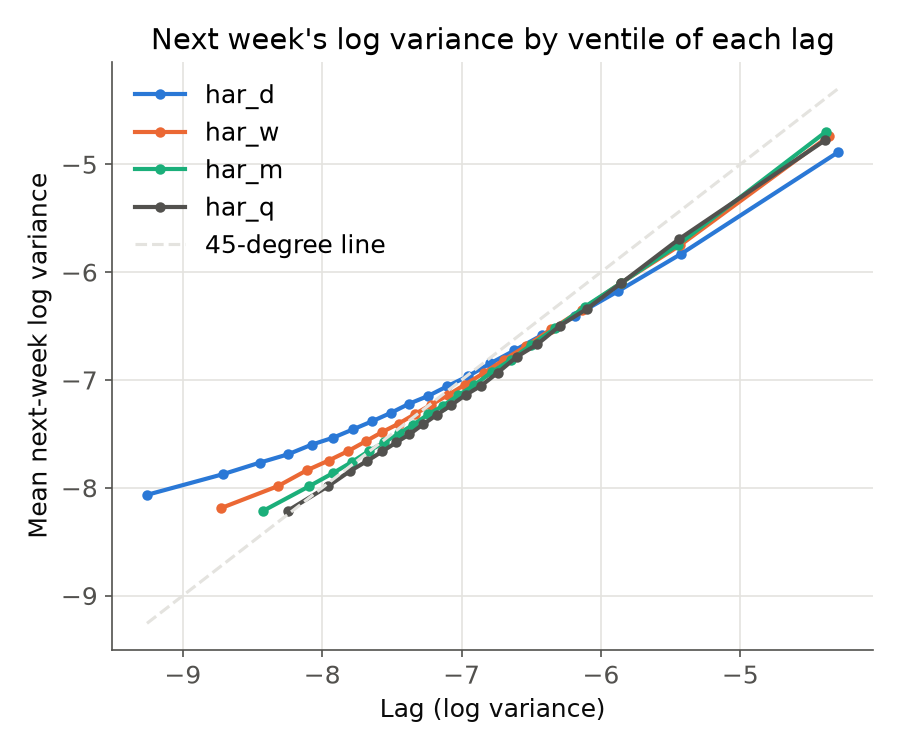
\includegraphics[width=\linewidth]{ms3_har_linearity.png}
    \column{0.58\textwidth}
    \footnotesize
    \begin{tabular}{@{}p{0.47\linewidth}p{0.47\linewidth}@{}}
      \toprule
      \textbf{Finding} (training years) & \textbf{Decision} \\
      \midrule
      target linear in each lag, slope $<1$ & linear HAR baselines; add \texttt{har\_q}, \texttt{har\_y} \\
      \addlinespace
      \nHeavy{} of \nNumeric{} features: excess kurtosis $> 10$ & map them to normal scores by rank \\
      \addlinespace
      range estimators correlate 0.96--0.99; VIX and 3-month VIX 0.98 & ridge and lasso, not OLS; ablation by block \\
      \addlinespace
      3-month VIX missing until 12/2007; no earnings data for delisted firms & impute 0, add a missing flag \\
      \addlinespace
      one stress week in validation & report validation by VIX level \\
      \bottomrule
    \end{tabular}\\[0.4em]
    All preprocessing is fit inside each training window (a scikit-learn \texttt{Pipeline}).
  \end{columns}
\end{frame}

%% =================================================================
%% Baselines
%% =================================================================
\begin{frame}{Baseline models: HAR fit three ways \speaker{Simon}}
  \footnotesize\setlength\tabcolsep{4pt}
  \begin{tabular}{@{}llll@{}}
    \toprule
    \textbf{Model} & \textbf{Inputs} & \textbf{Fit} & \textbf{Role} \\
    \midrule
    stock mean & company & training mean & the mean model \\
    \textbf{per-stock HAR}~\citep{corsi2009har} & day, week, month lags & OLS per company (52+ weeks) & \textbf{benchmark} \\
    pooled HAR & the same & one OLS & pooling alone \\
    pooled HAR + FE & the same & pooled slopes, company constant & + company level \\
    pooled HAR + market & + S\&P 500 variance, VIX & one OLS & + market \\
    GARCH(1,1)~\citep{bollerslev1986garch} & daily returns & MLE per company & classic model \\
    \bottomrule
  \end{tabular}
  \vspace{0.8em}
  \begin{columns}[T]
    \column{0.5\textwidth}
    \textbf{Training and validation}
    \begin{itemize}\setlength\itemsep{0.2em}
      \item each year 2016--2018 is forecast by a refit on all earlier rows
      \item 7-day embargo: a training target never reaches the forecast year
      \item the last 2018 Friday forecasts 2019, so it is a test row
      \item \ownFit{} of validation rows get their company's own HAR
    \end{itemize}
    \column{0.48\textwidth}
    \textbf{Metrics}
    \begin{itemize}\setlength\itemsep{0.2em}
      \item QLIKE~\citep{patton2011qlike} on the variance: robust to a noisy proxy
      \item MSE on the log variance
      \item DM test on weekly mean losses, Newey--West, HLN correction~\citep{harvey1997dm}
    \end{itemize}
  \end{columns}
\end{frame}

\begin{frame}{Baseline results: market information is what pooling adds \speaker{Simon}}
  \begin{columns}[c]
    \column{0.55\textwidth}
    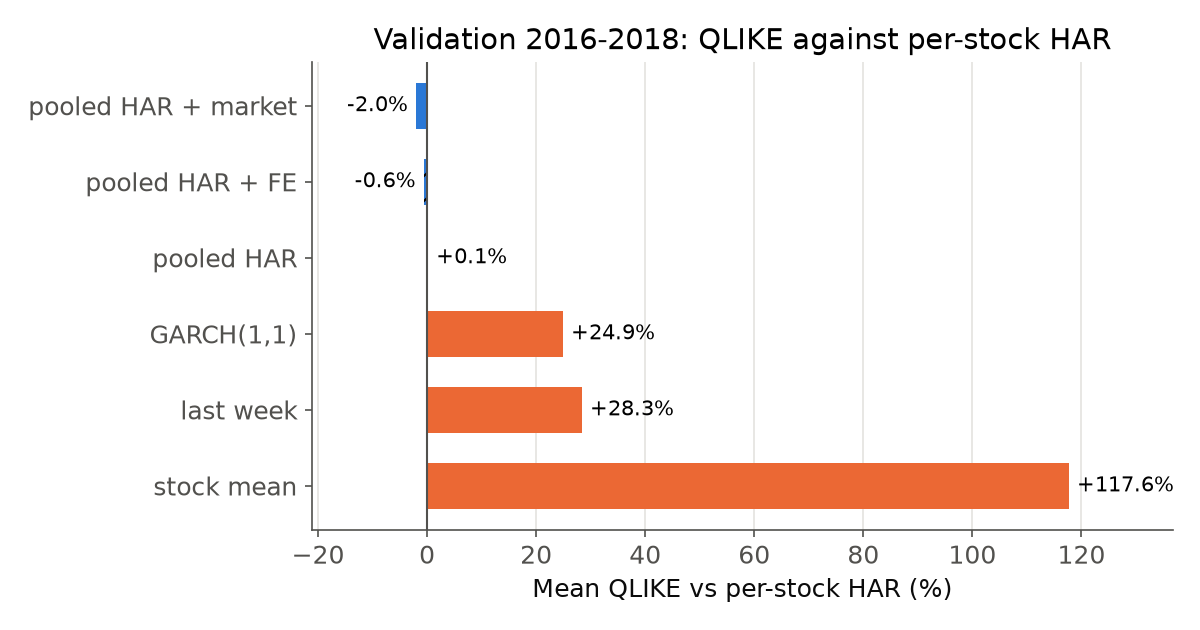
\includegraphics[width=\linewidth]{ms3_baselines.png}
    \column{0.43\textwidth}
    \small
    \begin{itemize}\setlength\itemsep{0.6em}
      \item \textbf{Per-stock HAR} is a strong benchmark: QLIKE \qlikeHar{}, MSE \mseHar{}.
            GARCH is \qGarch{} worse, the mean model \qStockMean{}.
      \item \textbf{Pooling alone} changes nothing: \qPooled{} ($p = \pPooled$).
      \item \textbf{Pooled HAR + market}: \qPooledMarket{} QLIKE ($p = \pPooledMarket$),
            \mPooledMarket{} MSE. Significant at 5\%.
      \item As in~\citet{zhang2024commonality}: pooling pays through what stocks share.
    \end{itemize}
  \end{columns}
\end{frame}

\begin{frame}{A first pooled model on every block: ridge and lasso \speaker{Shuo}}
  \begin{columns}[c]
    \column{0.58\textwidth}
    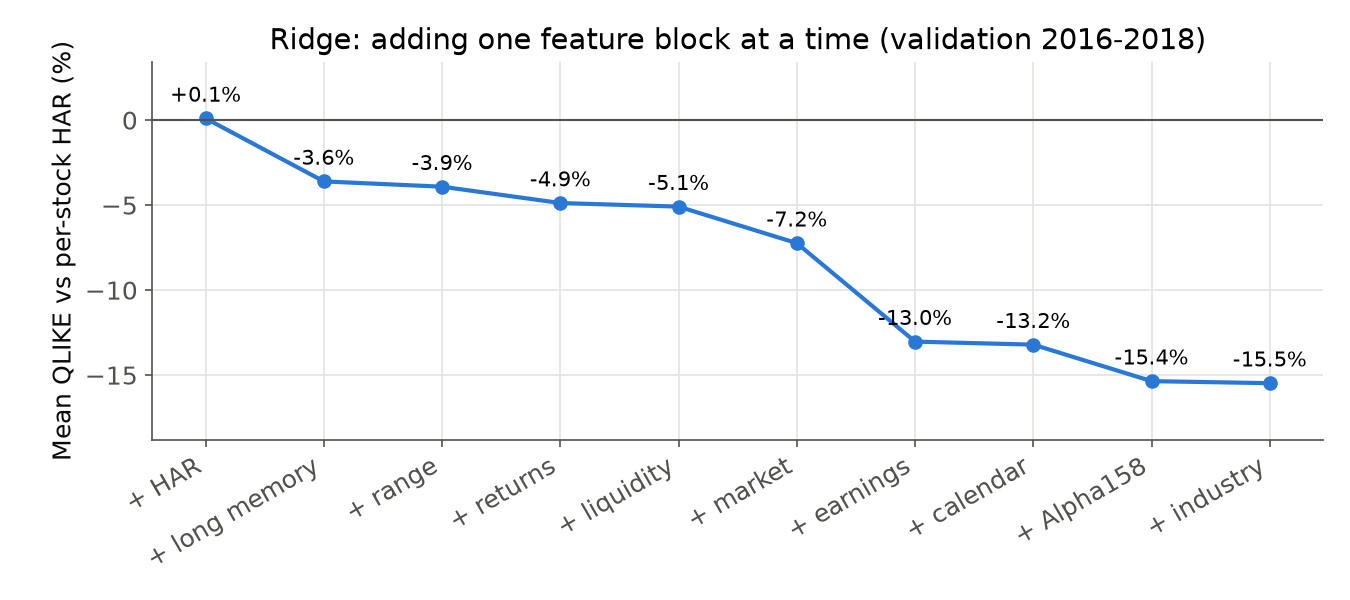
\includegraphics[width=\linewidth]{ms3_blocks.png}
    \column{0.4\textwidth}
    \small
    \begin{itemize}\setlength\itemsep{0.5em}
      \item \textbf{Ridge} ($\alpha = \ridgeAlpha$): \qRidge{} QLIKE, \mRidge{} MSE;
            \textbf{lasso} ($\alpha = \lassoAlpha$): \qLasso{}, keeps \lassoKept{} of
            \lassoInputs{} inputs. Penalty chosen on validation.
      \item \textbf{Blocks}: long memory \stepLong{}, + market \stepMarket{},
            + earnings \stepEarnings{} (the largest step), + Alpha158 \stepAlpha{}.
      \item Order matters: Q2 will drop one block at a time.
    \end{itemize}
  \end{columns}
\end{frame}

\begin{frame}{Where the models do well and where they do poorly \speaker{Terry}}
  \begin{columns}[c]
    \column{0.55\textwidth}
    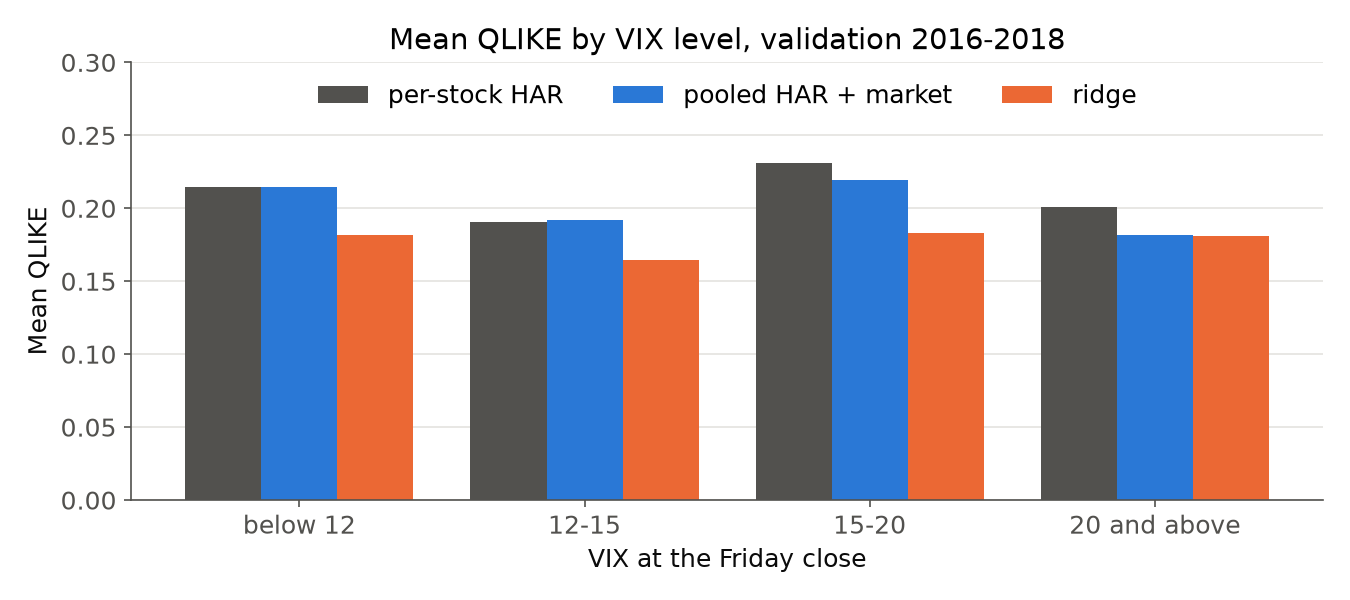
\includegraphics[width=\linewidth]{ms3_by_vix.png}\\[0.2em]
    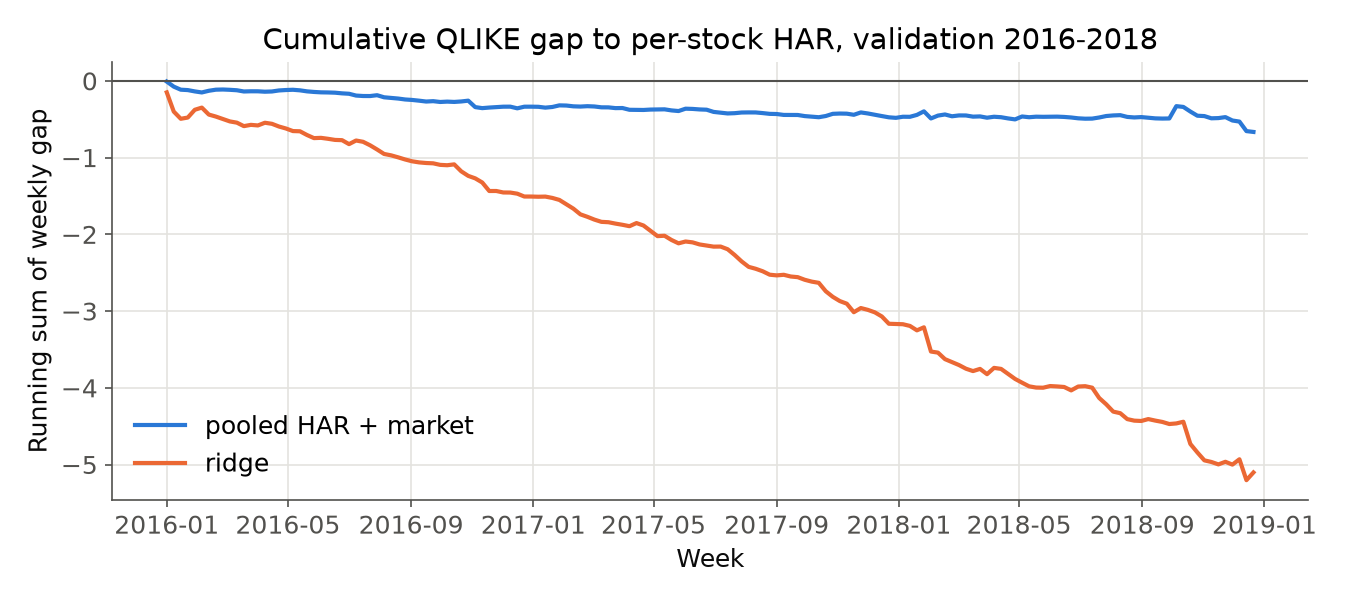
\includegraphics[width=\linewidth]{ms3_cumulative_gain.png}
    \column{0.43\textwidth}
    \footnotesize
    \textbf{Well}
    \begin{itemize}\setlength\itemsep{0.2em}
      \item earnings weeks: HAR's QLIKE \earnHar{} (\noEarnHar{} otherwise); ridge \earnRidge{}
      \item every volatility quintile; the gain builds up steadily over the three years
      \item calibrated: Mincer--Zarnowitz slope \mzRidge{} (HAR \mzHar{}), $R^2$ \rRidge{} vs \rHar{}
    \end{itemize}
    \textbf{Poorly}
    \begin{itemize}\setlength\itemsep{0.2em}
      \item VIX $\ge 20$ (\nHighVix{} rows): ridge \highVixRidge{} $\approx$ HAR + market \highVixMarket{}: ten blocks, no better than two inputs
      \item firms without SEC earnings data (survivorship): the earnings block changes QLIKE by only \leakBound{} there
    \end{itemize}
  \end{columns}
\end{frame}
\begin{frame}{The modeling pipeline for the final models \speaker{Terry}}
  \centering
  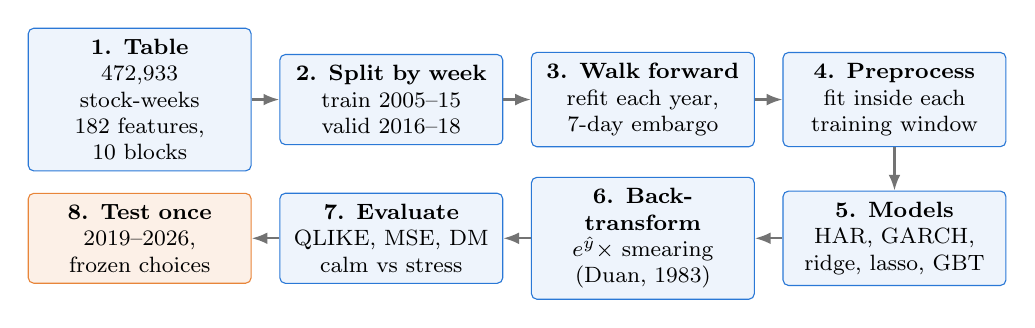
\begin{tikzpicture}[font=\footnotesize, node distance=0.28cm and 0.35cm,
      box/.style={draw=accent, fill=accent!8, rounded corners=2pt, align=center, inner sep=4pt,
                  minimum height=1.05cm, text width=2.55cm},
      hot/.style={box, draw=target, fill=target!12},
      arr/.style={-{Latex[length=2mm]}, thick, black!55}]
    \node[box] (data) {\textbf{1. Table}\\ \nRows{} stock-weeks\\ \nFeatures{} features, 10 blocks};
    \node[box, right=of data] (split) {\textbf{2. Split by week}\\ train 2005--15\\ valid 2016--18};
    \node[box, right=of split] (wf) {\textbf{3. Walk forward}\\ refit each year,\\ 7-day embargo};
    \node[box, right=of wf] (pre) {\textbf{4. Preprocess}\\ fit inside each\\ training window};
    \node[box, below=0.55cm of pre] (models) {\textbf{5. Models}\\ HAR, GARCH,\\ ridge, lasso, GBT};
    \node[box, left=of models] (back) {\textbf{6. Back-transform}\\ $e^{\hat y}\times$ smearing\\ (Duan, 1983)};
    \node[box, left=of back] (eval) {\textbf{7. Evaluate}\\ QLIKE, MSE, DM\\ calm vs stress};
    \node[hot, left=of eval] (test) {\textbf{8. Test once}\\ 2019--2026,\\ frozen choices};
    \foreach \a/\b in {data/split, split/wf, wf/pre, pre/models, models/back, back/eval, eval/test}
      \draw[arr] (\a) -- (\b);
  \end{tikzpicture}

  \vspace{0.5em}
  \raggedright\footnotesize
  \begin{columns}[T]
    \column{0.5\textwidth}
    \textbf{Tuned on validation}
    \begin{itemize}\setlength\itemsep{0.15em}
      \item ridge, lasso: penalty $\alpha$; tail threshold for normal scores
      \item GBT: learning rate, trees (early stopping), leaves, min leaf size, subsampling
      \item refit frequency, expanding vs rolling window; evolved factors kept
    \end{itemize}
    \column{0.48\textwidth}
    \textbf{Assumptions}
    \begin{itemize}\setlength\itemsep{0.15em}
      \item daily-range variance is a good proxy (0.95 corr.\ with 5-min RV)
      \item every feature is known by the Friday close (unit tests; rates lag a day)
      \item weekly mean loss gap is stationary (DM test)
    \end{itemize}
  \end{columns}
\end{frame}

%% =================================================================
%% Next steps
%% =================================================================
\begin{frame}{Next steps and questions for you \speaker{Ashley}}
  \begin{columns}[T]
    \column{0.5\textwidth}
    \textbf{Final models} (proposed owners)
    \small
    \begin{itemize}\setlength\itemsep{0.2em}
      \item gradient-boosted trees, tuned on validation: Ashley
      \item ridge and lasso with new market features (change in VIX, VIX term spread): Shuo
      \item HAR and GARCH on the test years, regime tables: Simon
      \item evaluation: Holm correction, model confidence set, stress split: Terry
      \item earnings dates for delisted firms, evolved-factor block, final notebook: Juntang
    \end{itemize}
    \column{0.48\textwidth}
    \textbf{Questions}
    \small
    \begin{enumerate}\setlength\itemsep{0.2em}
      \item Validation has \stressValid{} stress week (training \stressTrain{}). Is it fine that the
            stress results come only from the test years?
      \item Is reading the test years once, at the end, with every choice frozen, what you expect?
      \item Does the factor research (IC, genetic programming) count toward AC209A, next to the
            DM test?
      \item Train the final models on CRSP to 2025 (no survivorship before 2016)?
    \end{enumerate}
  \end{columns}
\end{frame}

%% =================================================================
%% Backup
%% =================================================================
\begin{frame}{Backup: every model on the validation years}
  \begin{columns}[c]
    \column{0.55\textwidth}
    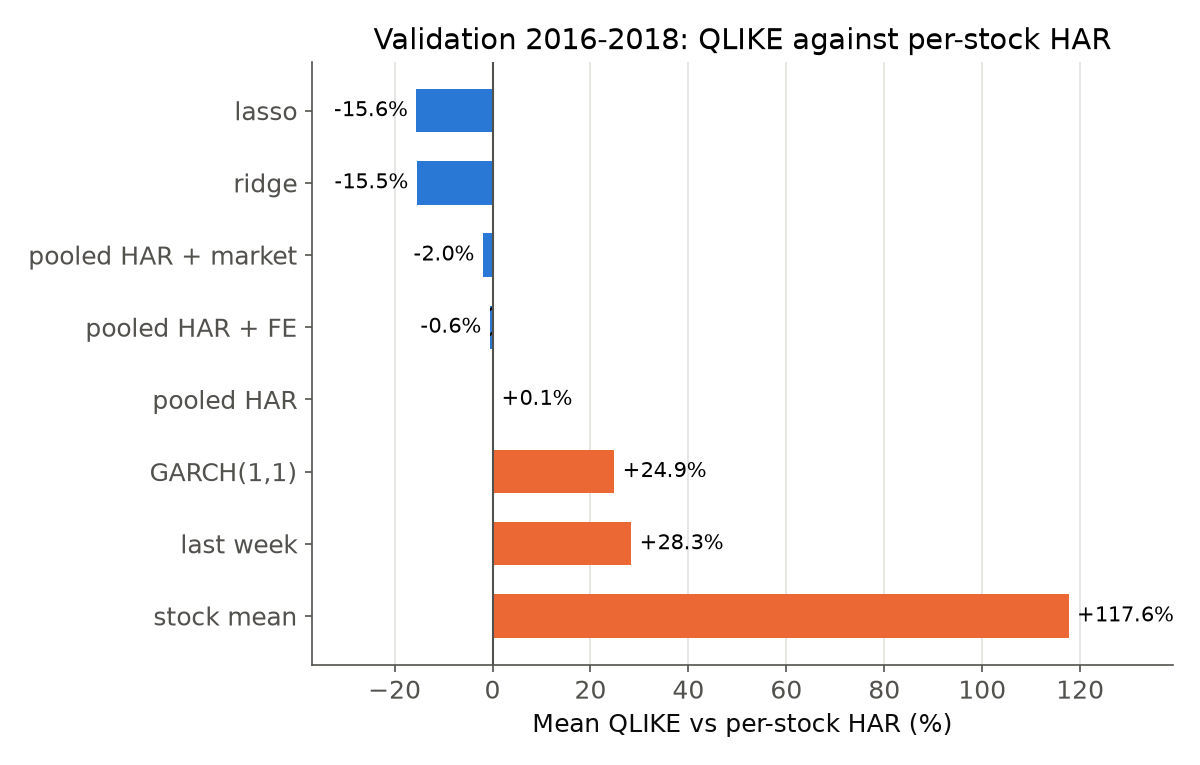
\includegraphics[width=\linewidth]{ms3_all_models.png}
    \column{0.43\textwidth}
    \footnotesize
    \setlength\tabcolsep{4pt}
    \begin{tabular}{@{}lrrr@{}}
      \toprule
      Model & QLIKE & MSE & $p$ (QLIKE) \\
      \midrule
      per-stock HAR & \qlikeHar{} & \mseHar{} & \\
      pooled HAR & \qPooled{} & \mPooled{} & \pPooled{} \\
      + FE & \qPooledFE{} & \mPooledFE{} & \pPooledFE{} \\
      + market & \qPooledMarket{} & \mPooledMarket{} & \pPooledMarket{} \\
      GARCH(1,1) & \qGarch{} & \mGarch{} & \pGarch{} \\
      ridge & \qRidge{} & \mRidge{} & \pRidge{} \\
      lasso & \qLasso{} & \mLasso{} & \pLasso{} \\
      \bottomrule
    \end{tabular}\\[0.4em]
    Change against per-stock HAR; hatched: not significant at 5\%.
  \end{columns}
\end{frame}

\begin{frame}{Backup: calibration and the fitting scheme}
  \begin{columns}[c]
    \column{0.42\textwidth}
    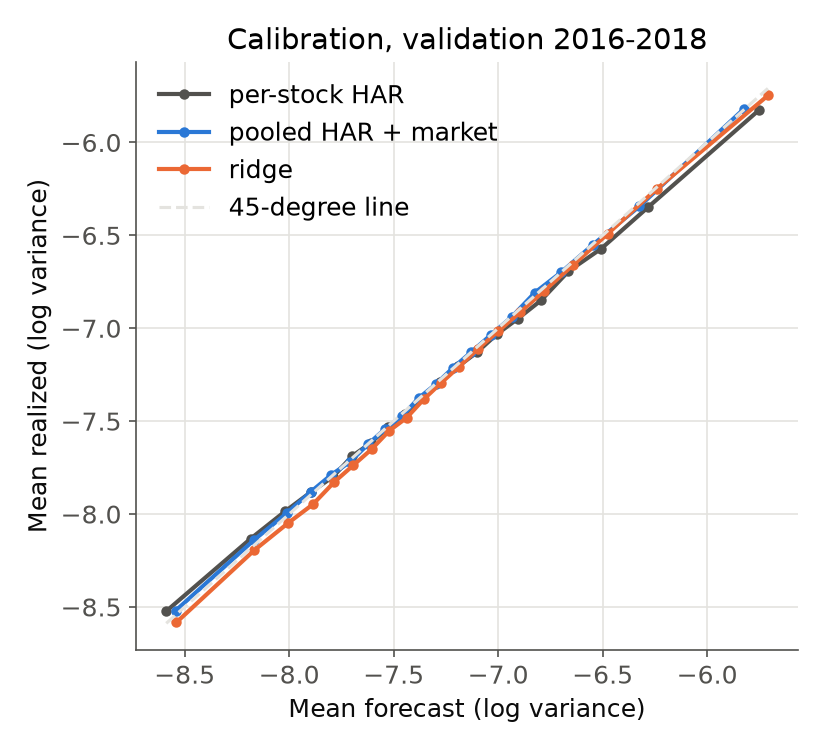
\includegraphics[width=\linewidth]{ms3_calibration.png}
    \column{0.56\textwidth}
    \small
    \begin{itemize}\setlength\itemsep{0.6em}
      \item Binned forecasts lie on the 45-degree line for all three models.
      \item \textbf{Fitting scheme}~\citep{audrino2024hard}: quarterly refits give the same QLIKE as yearly
            ones; a 5-year rolling window is slightly worse than expanding. Weekly HAR, unlike
            daily HAR, does not need frequent refits.
      \item \textbf{Second evolved factor}: weekly variance over $\sqrt{\text{volume volatility}}$,
            IC \evolvedTwoTrain{} in training, \evolvedTwoValid{} on validation.
    \end{itemize}
  \end{columns}
\end{frame}

\begin{frame}[allowframebreaks]{References}
  \footnotesize
  \bibliographystyle{unsrtnat}
  \bibliography{ref}
\end{frame}

\end{document}
